\chapter{Definición del Producto y Requerimientos}

\section{Requerimientos Funcionales}

Los requerimientos funcionales de un proyecto de software son las descripciones de las funcionalidades que deberá realizar el mismo. Se refiere tanto al manejo de datos como a las acciones que el usuario puede ejecutar sobre el programa. Estos requerimientos se definen para permitir la implementación de la solución. A continuación, se detallan las historias de usuario de Nidio, explicaciones cortas que siguen un formato definido de las funciones de la plataforma, desde el punto de vista del usuario final.

\subsection{Épicas}

Las historias de usuario llamadas épicas son las que, generalmente, se realizan a más alto nivel y no incluyen detalles.

\subsubsection{Autenticación de Usuarios}

\begin{itemize}
\item Como usuario quiero poder crear una cuenta en Nidio y acceder a ella con mis credenciales para utilizar las herramientas de análisis inmobiliario de forma personalizada.
\end{itemize}

\subsubsection{Valuación de Propiedades}

\begin{itemize}
\item Como usuario quiero poder ingresar las características de una propiedad y obtener un rango de precio estimado para evaluar si su precio de mercado es coherente con el valor real.
\end{itemize}

\subsubsection{Visualización Geoespacial de Precios}

\begin{itemize}
\item Como usuario quiero poder explorar mapas de calor de precios por metro cuadrado, niveles de ruido y condiciones de seguridad en CABA para comprender la distribución territorial del mercado inmobiliario y evaluar el entorno de las propiedades que estoy considerando.
\end{itemize}

\subsubsection{Life Score}

\begin{itemize}
\item Como usuario quiero poder obtener un indicador de entorno urbano para una propiedad seleccionada para evaluar la calidad de su entorno en función de la proximidad a puntos de interés relevantes.
\end{itemize}

\subsubsection{Exploración de Propiedades}

\begin{itemize}
\item Como usuario quiero poder explorar un catálogo de propiedades con filtros por tipo, barrio, operación y precio para identificar opciones de interés y analizarlas con las herramientas de valuación y entorno de la plataforma.
\end{itemize}

\subsection{Historias de Usuario}

\subsubsection{Épica 1 --- Autenticación de Usuarios}

\begin{itemize}
\item \textbf{HU-01:} Como usuario quiero poder registrarme con nombre, email y contraseña para crear una cuenta en Nidio y acceder a sus funcionalidades.
\item \textbf{HU-02:} Como usuario quiero poder iniciar sesión con mi email y contraseña para acceder a mi cuenta.
\item \textbf{HU-03:} Como usuario quiero poder recuperar mi contraseña mediante un enlace enviado a mi email para recuperar el acceso a mi cuenta en caso de olvidarla.
\item \textbf{HU-04:} Como usuario quiero poder cerrar sesión para proteger el acceso a mi cuenta.
\end{itemize}

\subsubsection{Épica 2 --- Valuación de Propiedades}

\begin{itemize}
\item \textbf{HU-05:} Como usuario quiero poder seleccionar el tipo de operación (compra o alquiler) y el tipo de propiedad (departamento, casa o PH) antes de ingresar los datos de valuación para obtener una estimación adecuada al segmento correspondiente.
\item \textbf{HU-06:} Como usuario quiero poder ingresar la superficie, el barrio, la cantidad de ambientes y el tipo de propiedad para obtener un rango de precio estimado por el modelo de valuación.
\item \textbf{HU-07:} Como usuario quiero poder visualizar el rango de precio estimado junto con una indicación de si el precio de mercado declarado está dentro, por encima o por debajo del rango esperado para identificar posibles sobrevaluaciones o subvaluaciones.
\end{itemize}

\subsubsection{Épica 3 --- Visualización Geoespacial de Precios}

\begin{itemize}
\item \textbf{HU-08:} Como usuario quiero poder visualizar un mapa de calor de precios por metro cuadrado en CABA para comprender la distribución geográfica del mercado inmobiliario.
\item \textbf{HU-09:} Como usuario quiero poder filtrar el mapa de calor por tipo de operación (compra o alquiler) para ver la distribución de precios correspondiente al segmento de mi interés.
\item \textbf{HU-10:} Como usuario quiero poder hacer clic sobre una zona del mapa para ver el precio promedio por metro cuadrado en ese barrio.
\item \textbf{HU-11:} Como usuario quiero poder visualizar un mapa de calor de niveles de ruido por zona en CABA para evaluar el entorno sonoro de las propiedades que estoy considerando.
\item \textbf{HU-12:} Como usuario quiero poder visualizar un mapa de calor de condiciones de seguridad por zona en CABA basado en registros de hurtos y robos para evaluar la seguridad del entorno de las propiedades que estoy considerando.
\end{itemize}

\subsubsection{Épica 4 --- Life Score}

\begin{itemize}
\item \textbf{HU-13:} Como usuario quiero poder ingresar la dirección de una propiedad para obtener su Life Score y conocer la calidad de su entorno urbano.
\item \textbf{HU-14:} Como usuario quiero poder puntuar cada una de las siete categorías de POIs según su importancia personal para obtener un Life Score adaptado a mis preferencias.
\item \textbf{HU-15:} Como usuario quiero poder ver en un mapa los puntos de interés cercanos a la propiedad seleccionada para tener una referencia visual del entorno evaluado.
\end{itemize}

\subsubsection{Épica 5 --- Exploración de Propiedades}

\begin{itemize}
\item \textbf{HU-16:} Como usuario quiero poder explorar un catálogo de propiedades con filtros por tipo de propiedad, barrio, tipo de operación y rango de precio para identificar opciones que se ajusten a mis criterios de búsqueda.
\item \textbf{HU-17:} Como usuario quiero poder acceder al detalle de una propiedad del catálogo para ver su información completa junto con su valuación estimada y su Life Score.
\item \textbf{HU-18:} Como usuario quiero poder ingresar una dirección y ver las propiedades del catálogo ubicadas dentro de un radio máximo de 2 kilómetros para encontrar opciones cercanas a una zona de mi interés.
\end{itemize}

\section{Requerimientos No Funcionales}

Los requerimientos no funcionales describen los estándares de calidad bajo los cuales el sistema debe operar. Para su definición se adopta el modelo ISO/IEC 25010 (SQuaRE), que establece ocho características de calidad de producto.

\subsection{Adecuación Funcional}

\begin{itemize}
\item La plataforma debe proveer estimaciones de precio coherentes con los datos de entrenamiento del modelo para propiedades ubicadas en CABA.
\item El Life Score debe reflejar correctamente la proximidad a las categorías de POIs definidas dentro del radio establecido.
\end{itemize}

\subsection{Eficiencia de Rendimiento}

\begin{itemize}
\item La plataforma debe responder a las consultas de valuación en un tiempo menor a 5 segundos.
\item Los mapas de calor deben cargarse en un tiempo menor a 3 segundos.
\item El cálculo del Life Score debe completarse en un tiempo menor a 5 segundos.
\item La plataforma debe soportar al menos 50 usuarios concurrentes sin degradación del servicio. Este umbral fue definido como un objetivo realista y medible para un MVP, consistente con el alcance del prototipo y el contexto de despliegue en infraestructura cloud básica.
\end{itemize}

\subsection{Compatibilidad}

\begin{itemize}
\item La plataforma debe ser compatible con los navegadores Google Chrome, Mozilla Firefox, Safari y Microsoft Edge en sus versiones actuales.
\item Los servicios del sistema deben poder integrarse entre sí mediante interfaces REST bien definidas.
\end{itemize}

\subsection{Usabilidad}

\begin{itemize}
\item La interfaz debe ser intuitiva y no requerir capacitación previa para su uso.
\item La plataforma debe ser responsiva y funcionar correctamente en dispositivos de escritorio y móviles.
\item Los resultados de valuación y el Life Score deben presentarse de forma clara y comprensible para usuarios sin conocimientos técnicos.
\end{itemize}

\subsection{Confiabilidad}

\begin{itemize}
\item La plataforma debe estar disponible las 24 horas los 7 días de la semana.
\item El sistema debe poder reiniciarse automáticamente ante fallos sin pérdida de datos.
\item Los datos de la base de datos deben contar con respaldos periódicos para garantizar su recuperación ante fallos.
\item El sistema debe contemplar un período de mantenimiento programado en horarios de baja actividad.
\end{itemize}

\subsection{Seguridad}

\begin{itemize}
\item Las contraseñas de los usuarios deben almacenarse cifradas mediante un algoritmo de hashing seguro.
\item La comunicación entre el cliente y el servidor debe realizarse mediante protocolo HTTPS.
\item El acceso a las funcionalidades de análisis debe requerir autenticación previa.
\item Los tokens de sesión deben tener un tiempo de expiración definido.
\end{itemize}

\subsection{Mantenibilidad}

\begin{itemize}
\item La arquitectura del sistema debe estar desacoplada en servicios independientes (frontend, backend, microservicio Python) para facilitar el mantenimiento y la actualización de cada componente.
\item El modelo de valuación debe poder ser reentrenado y reemplazado sin interrumpir el servicio.
\item El código fuente debe estar documentado y versionado en un repositorio de control de versiones.
\end{itemize}

\subsection{Portabilidad}

La plataforma debe funcionar correctamente en los sistemas operativos Windows, macOS y Linux desde el navegador, sin requerir instalación de software adicional por parte del usuario.

\subsection{Estrategia de Validación}

La validación de los requerimientos no funcionales se llevará a cabo de forma integral durante la fase de pruebas del proyecto. La adecuación funcional se verificará mediante pruebas que comparen las estimaciones del modelo contra valores de referencia del mercado y que confirmen que el Life Score refleja correctamente los POIs dentro del radio definido. La eficiencia de rendimiento se validará mediante pruebas de carga simulando 50 usuarios concurrentes y midiendo los tiempos de respuesta de cada componente. La compatibilidad se verificará mediante pruebas manuales en los navegadores definidos sobre dispositivos de escritorio y móviles. La usabilidad se evaluará con personas representativas de los tres perfiles definidos en el User Research. La confiabilidad se monitoreará a través del uptime del servicio durante el período de evaluación mediante las herramientas del proveedor cloud. La seguridad se validará mediante pruebas funcionales sobre autenticación, cifrado de contraseñas, protocolo HTTPS y expiración de tokens. La mantenibilidad se verificará mediante la correcta separación de servicios y la documentación del código en el repositorio de control de versiones. Finalmente, la portabilidad se validará mediante pruebas de despliegue en el entorno cloud seleccionado verificando su correcto funcionamiento en distintos sistemas operativos y navegadores.

\clearpage
\section{Viabilidad y Gestión del Proyecto}

\subsection{Cronograma de Actividades (Gantt)}

\begin{figure}[H]
\centering
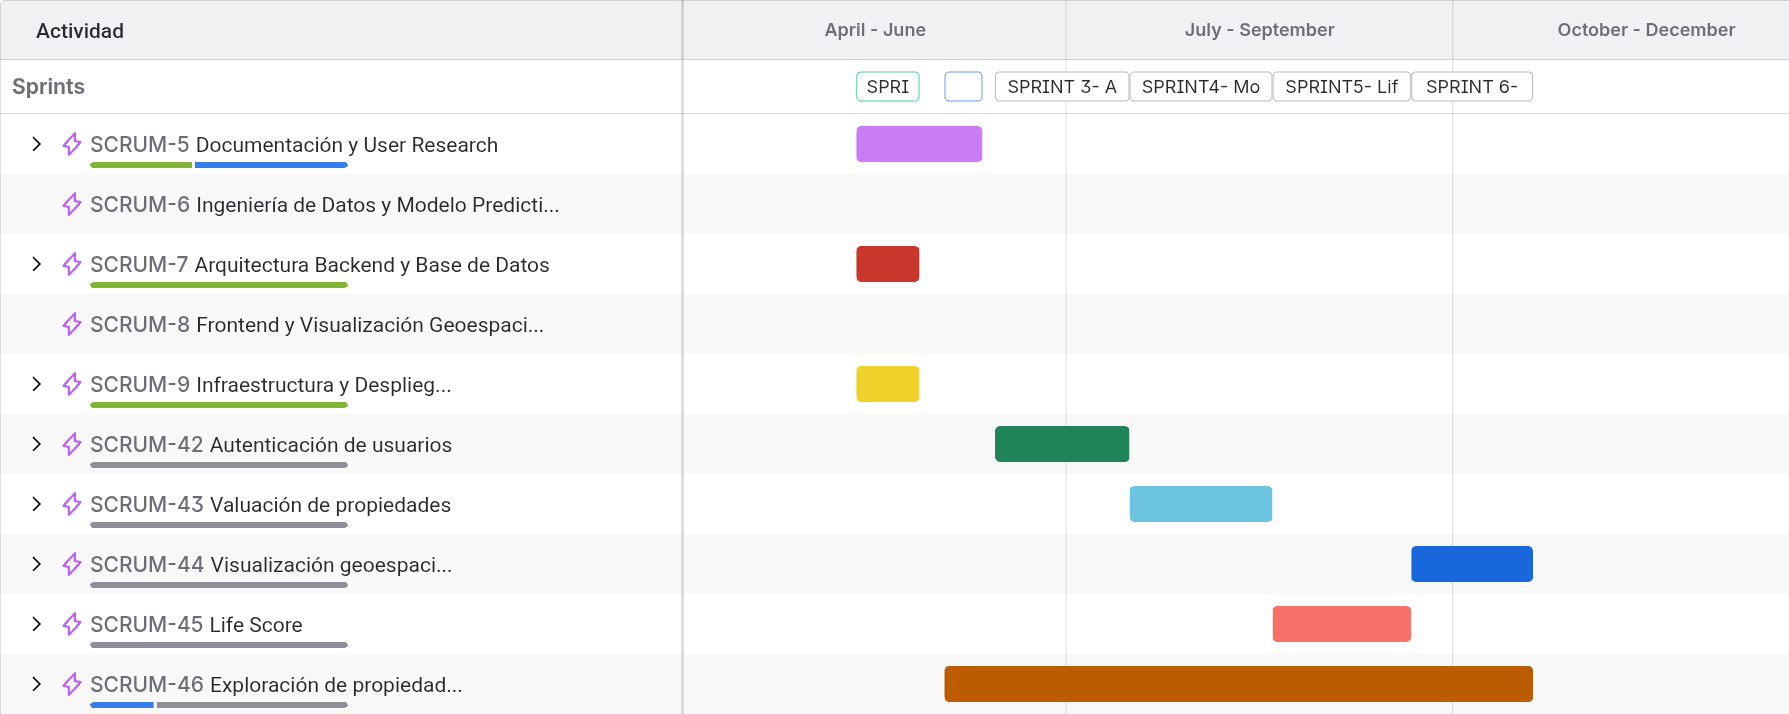
\includegraphics[width=0.90\textwidth]{figures/word/image1.png}
\caption{Cronograma de actividades del proyecto.}
\end{figure}

\nocite{AbidoyeChan2018,Akerlof1970,Argenprop2026,ArgentinaLey25326,Babtan2024,BaumEtAl2020,BirkelandEtAl2021,Boeing2019,BraesemannBaum2020,ColegioEscribanos2026,DrojEtAl2024,ElJaouhariEtAl2024,FaxvaagEtAl2025,GlumacDesRosiers2018,BADataDelitos,BADataMapaRuido,GutierrezEtAl2025,ISO25010,JLL2024,KokEtAl2017,LundbergLee2017,Malczewski2006,PivoFisher2011,Rosen1974,SiniakEtAl2020,SoltanaEtAl2017,StangEtAl2021,Szwoch2019,TagliaroEtAl2024,Zonaprop2026}
